\listfiles
\documentclass[twoside,12pt]{article}
\newcommand{\dataset}{{\cal D}}
\newcommand{\fracpartial}[2]{\frac{\partial #1}{\partial  #2}}
\usepackage{hyperref}
\usepackage{enumerate}
\usepackage[top=2in, bottom=1.5in, left=0.85in, right=0.5in]{geometry}
\usepackage[hyphenbreaks]{breakurl}
%\usepackage[pdfstartview=FitH,pdfstartpage=13,pdfpagemode=UseNone]{hyperref}
\usepackage{amsfonts}
\usepackage{graphicx} 
\usepackage[linesnumbered,ruled]{algorithm2e}
\usepackage{float}
\usepackage{amssymb,amsmath}
\usepackage{mdwlist }
\usepackage{color}
\usepackage{multirow}
\usepackage{listings}
\usepackage{float}
\usepackage{setspace}
\usepackage[english]{babel}

\usepackage{graphicx}
\usepackage{caption}
\usepackage{subcaption}


\definecolor{darkblue}{rgb}{0.0,0.0,0.5}
\newtheorem{Dfn}{Definition}
\hypersetup{colorlinks,breaklinks,
            linkcolor=darkblue,urlcolor=darkblue,
            anchorcolor=darkblue,citecolor=darkblue}
\newcommand{\sign}{\text{sign}}
\newcommand{\argmin}{\arg\!\max}
\begin{document}

\title{Recursive Auto Encoder (RAE)
Method of Learning Meanings for Sentences\\  Learning Algorithms, Project 4}
\author{Mohsen Malmir, Erfan Sayyari}
\maketitle

\section*{Abstract}
In this paper, we develop a recursive auto encoder neural network for recognizing sentence level sentiment. A difficulty arises when input to neural networks is text sentence. In this paper, we choose a dynamic representation for sentences that is derived greedily to minimize the reconstruction error. This sentence level representation dictates the form of shape of the neural network. We also adapt a flexible representation for words that resembles the meaning of that word in a low dimensional space. The word representations  update as recognition error back propagates through the auto-encoder neural network. We demonstrate the performance of the proposed model on the movie review dataset \cite{pang2005}. This is a dataset that contains "positive" and "negative" reviews of movies, each comprised of one or more sentences. Our model can produce comparable results on this dataset.

\section{Introduction}
One of the main challenges in text-related applications of machine learning is the representation of the data. In applications such as topic modeling, an input corpus is represented by a bag-of-words model, which ignores the basic property that comprises the text: order of the words. One way to deal with this is to use \emph{n-grams}, which builds a representation of the text based on n-consecutive words in sentences. However, to avoid the curse of dimensionality, this approach is applied only with small values of n, which is insufficient in the applications such as extracting meaning of the text.

With increasing volume and importance of online reviews, predicting \emph{sentiment} is becoming crucial for understanding the user generated content on websites. The baseline method for this task is to use a bag-of-words representation \cite{pang2002}. These methods fail to capture the sentiment properly, as they ignore words order, a crucial component in analyzing text. For example in reviews about a movie, "A good movie from a bad director" has actually positive sentiment, but "A bad movie from a good director" has negative sentiment, considering the target is reviews about the movie.

In this paper, we develop a representation for text sentences that is based on individual words \emph{meanings}. The meaning of sentence is constructed based on the meaning of individual words and their order in the sentence. This requires representation of meaning in someway, however is no standard way to do this without falling into philosophical issues. We choose a $d$-dimensional real valued vector for to represent meaning of parts of text. A good candidate to combine the meaning of words to get sentence level meaning is to use the sentence's parse tree. However this requires use of some external text processing package which means the results can't be generalized to other languages. In this paper, we introduce a greedy approach to combine meanings of parts of text based on the concept of auto encoder neural network. The benefits of this approach is its speed and that it can be generalized to other languages with no extra effort. We show that this greedy method is capable of producing state of the art results for sentiment prediction task on a movie review dataset.

The main contributions of this paper are introducing a compositional structure to represent meaning of text and developing a greedy method to implement this structure. A recursive auto encoder neural network is used to combine the meanings of parts of sentence by minimizing the reconstruction error. At the top level, meaning of sentence is used in a \emph{softmax} classifier to predict the sentiment. We show that this model can achieve state-of-the-art performance on sentiment prediction of the movie review dataset.

\section{Proposed Model}
\subsection{Overal Architecture}
An exemplar architecture of the proposed model is shown in figure \ref{figRAE}. In this figure, the input sentence has 4 words which are shown in the bottom level of the network with blue nodes. Each word is represented by a $d$-dimensional vector representing its meaning. The orange nodes indicate the composition nodes which are constructed by \emph{encoding} the meaning of two words of parts of sentence. Matrix $W^1$ with size $2d \times d$ at each orange node indicates the meaning-composition stage of the network. For the composition of meanings to be appropriate, a \emph{reconstruction} stage is added that is shown by violet nodes. Matrix $W^2$ with size $d\times 2d$ is used to reconstruct the original meaning vectors from a composite meaning. Note that the same matrices are used in all levels of encoding and reconstruction in the network. A prediction stage is added to the top level meaning node of the network, shown in green. For a target value of dimensionality $k$, a prediction matrix $W^{label}$ with size $d \times k$ is used which transforms the meaning to the input of a softmax function with $k$ target classes.

\begin{figure}[ht!]
\centering
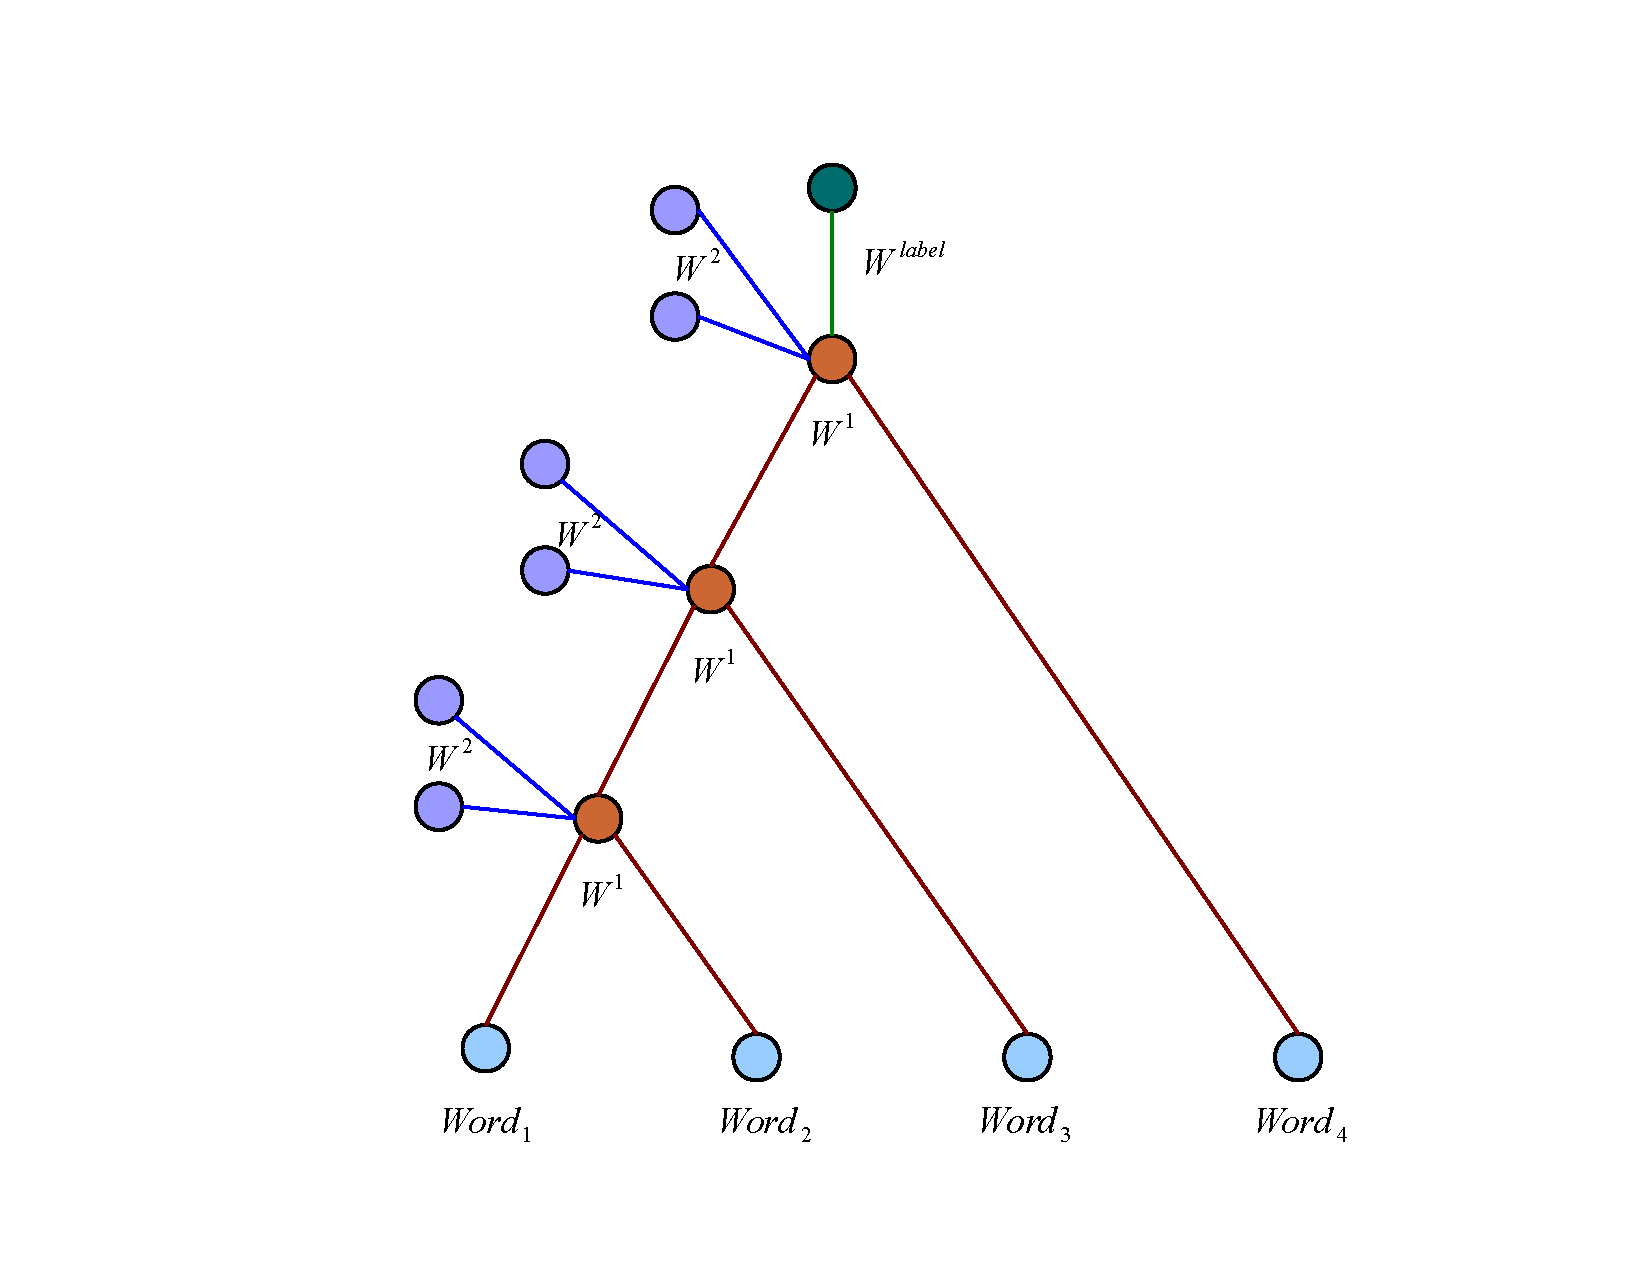
\includegraphics[width=.8\textwidth]{raenet.pdf}
\caption{An exemplar schematic diagram of recursive auto-encoder network developed in this paper. Blue nodes indicate the words of the input sentence, the orange nodes indicate the intermediate coding of meaning of parts of sentence. The violet nodes are the reconstruction of input nodes, and the green node is the predicted target. The weight matrices for encoding, reconstruction and label prediction are indicated correspondingly by $W^1$, $W^2$ and $W^{label}$. }
\label{figRAE}
\end{figure}


A more detailed view of the encoding and reconstruction stages is shown in figure \ref{figEncodingDecoding}. This is called an auto-encoder network. The goal of encoding is to produce a $d$-dimensional representation $Z$ from two $d$-dimensional meaning vectors, shown by $X$ and $Y$. The encoded representation $Z$ is calculated by,
\begin{equation}
Z = h(W^1 [X;Y] + b^1)
\label{eqEncoding}
\end{equation}
where $W^1$ is a $d\times 2d$ matrix, $b^1$ is a $d\times 1$ vector, $h$ is a point-wise thrashing function $h: \mathbb{R}^d \rightarrow \mathbb{R}^d$ and $[X;Y]$ indicates the column-wise concatenation of vectors $X$ and $Y$, that is $X$ and $Y$ are $d\times 1$ vectors and $[X;Y]$ is a $2d\times 1$ vector. The purpose of encoding stage is to produce a representation that is the composite of meanings of individual elements of the sentence. By using only two inputs for encoding, we are putting constraints on the model that simplifies the implementation. One should note that though the meaning of a phrase is well defined in traditional view of meaning, longer expression's or sentence's meaning that is acquired in our model is only interpretable in the context of overall goal of the network, which is in this case predicting the sentiment.

Having a composite meaning vector $Z$, a measure of goodness of encoding is to reconstruct the original meaning vectors by an inverse transformation. This is shown using blue lines and violet nodes in figure \ref{figEncodingDecoding}. Specifically, having vector $Z$, we can transform it back to reconstructions $X'$ and $Y'$ using,
\begin{equation}
[X',Y'] = W^2 Z + b^2
\label{eqReconst}
\end{equation}
where $W^2$ is a $2d\times d$ matrix, $b^2$ is a $2d\times 1$ vector and $X'$ and $Y'$ are $d\times 1$ vectors. The encoding and decoding stages together comprise a single orange node in figure \ref{figRAE}. Note that the same parameters ($W^1,W^2,b^1,B^2$ and $h$) are used in different orange nodes of the tree. Starting from the lowest orange node, a compact meaning is derived from its inputs, which is then fed to the orange node in the next level to be combined with other compact meanings of the parts of sentence. This is repeated until a single $d$ dimensional vector representation is produced for the sentence. For now, consider that the structure of the tree is given. Later in this section, we will delve into the details of calculating the structure of tree for different sentences.

\subsection{Reconstruction Error}
The goal of the auto-encoder network is to produce  a compact representation of the inputs, which is good enough to be used to decode the original vectors. We define the \emph{reconstruction error} of the auto-encoder as,
\begin{equation}
E_{rec}(X,Y,X',Y') = \frac{n_X}{n_X+n_Y}||X-X'||^2+\frac{n_Y}{n_X+n_Y}||Y-Y'||^2
\label{eqRecErr}
\end{equation}
Here, $n_X$ and $n_Y$ are the length of the parts of the input sentence that are encoded in $X$ and $Y$ correspondingly. For leaf nodes, $n_X$ is equal to 1. For non-leaf nodes, $n_X = n_{lc} + n_{rc}$ where $n_{lc}$ and $n_{rc}$ are the corresponding $n$ for left and right child of $X$. We use the reconstruction error to train the parameters $W^1,W^2,b^1,b^2$.



\begin{figure}[ht!]
\centering
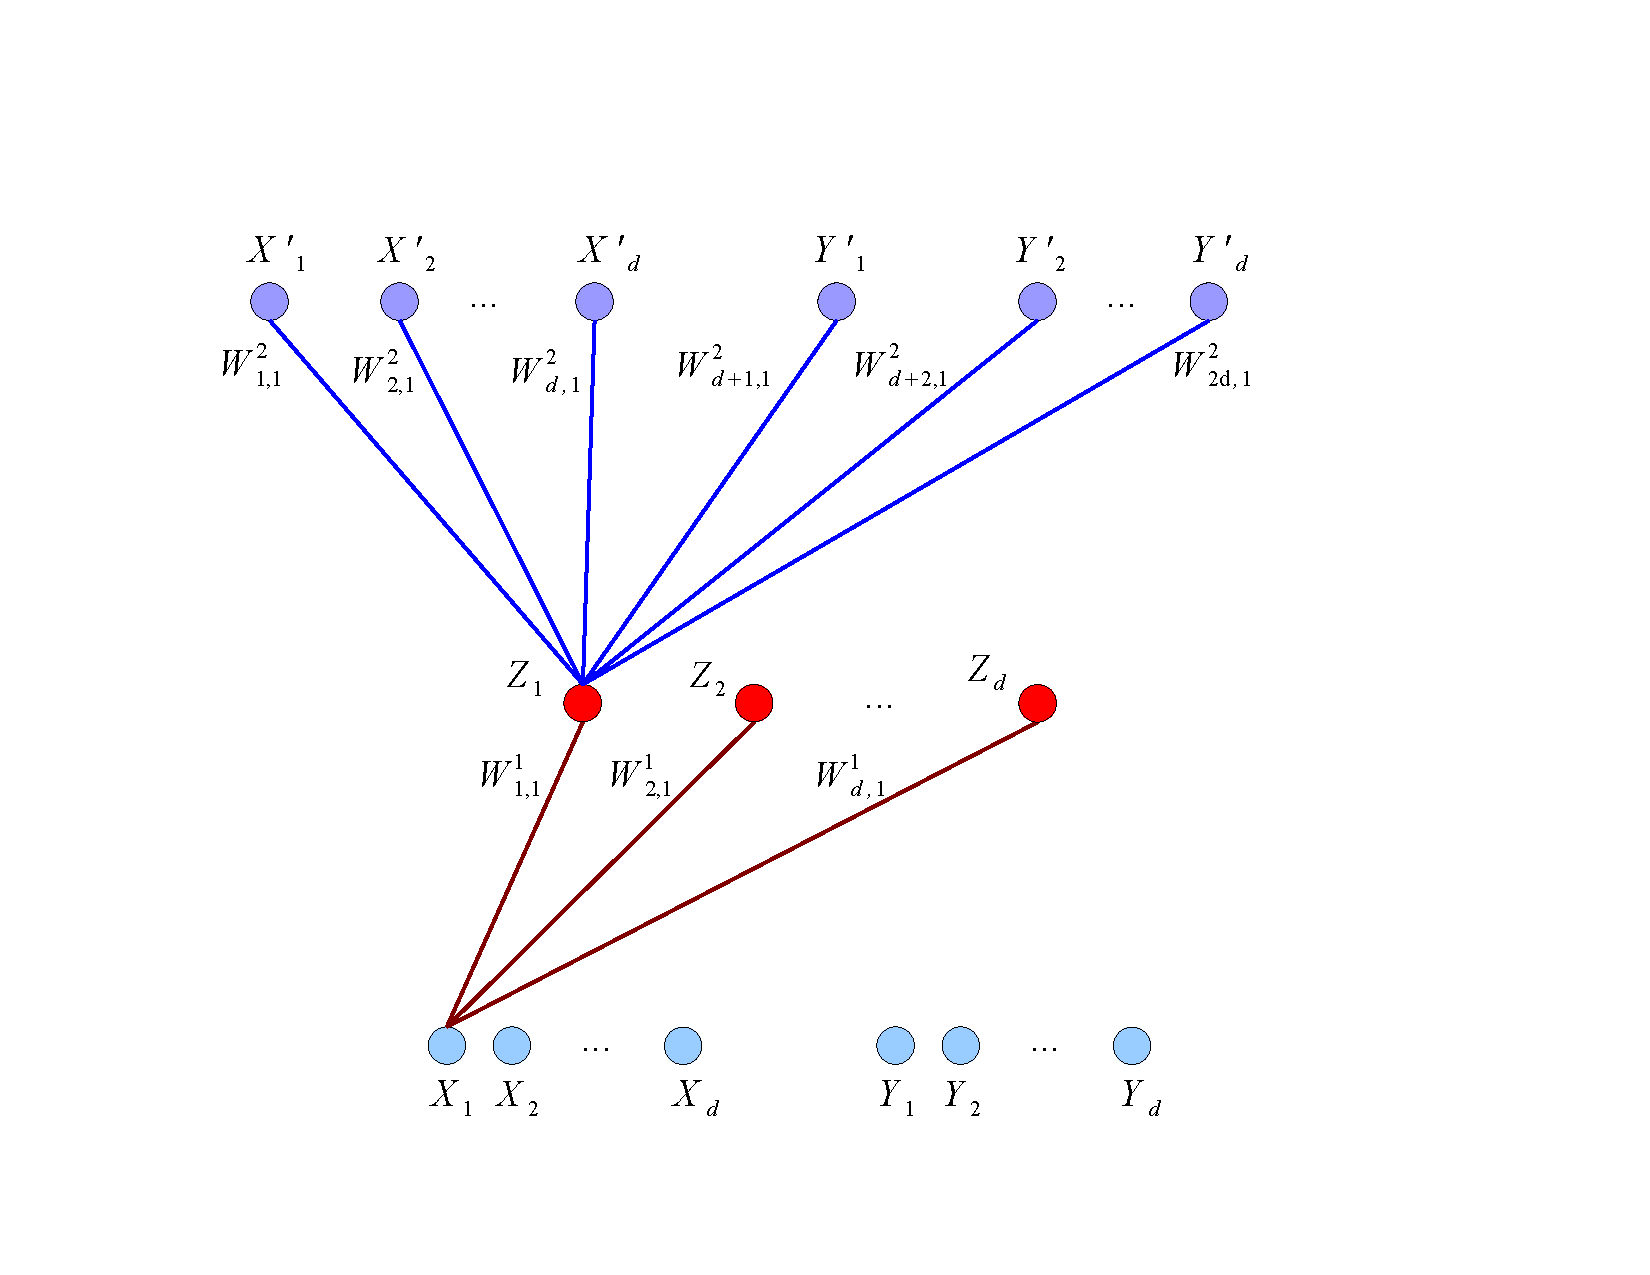
\includegraphics[width=.8\textwidth]{autoencoder.pdf}
\caption{Encoding and Decoding stages of the recursive auto-encoder network. There are two $d$-dimensional inputs to the network. The encoding part which is indicated by matrix $W^1$ and red-colored edges,  embeds the inputs to a $d$-dimensional representation. The decoding stage is represented by blue color edges and matrix $W^2$, aims to reconstruct the original inputs from the encoded representation. Only one column of $W^1$ and $W^2$ are shown for clarity.}
\label{figEncodingDecoding}
\end{figure}


\subsection{Predicting Sentiment}
We use the top level meaning to predict the sentiment of the sentence. This is indicated by the green edge and node in figure \ref{figRAE}. Let $Z$ denote the top-level meaning of the sentence, then
\begin{equation}
V = \text{softmax}(W^{label} Z)
\end{equation}
denotes the predicted sentiment for the input sentence. $W^{label}$ is a $K\times d$ matrix, which transforms the $d$-dimensional meaning vector into a $K$-dimensional vector. The softmax function for an input of size $K$ is defined as,
\begin{equation}
V_k = \frac{e^{W^{label}_{k,:}Z}}{\sum_{i=1}^K e^{W^{label}_{i,:}Z}}
\end{equation}
where $W^{label}_{j,:}$ indicates the $j$th row of the matrix $W^{label}$. Each training sentence is accompanied by a vector $T$ of length $K$ of target values. We use the cross entropy between the target value and the predicted value as a measure of error,
\begin{equation}
E_{CE} (T,V|\theta) = -\sum_{i=1}^K -T_i \log V_k
\label{eqCEErr}
\end{equation}
here, $\theta$ indicates the model. We use back propagation to update the model parameters.

\subsection{Greedy Construction of Neural Network Structure}
Up to now, we assumed that the tree structure of the neural network is given. In this section, we develop a greedy algorithm to construct this tree. In order to understand this step clearly, we should note that the tree structure dictates the way the meaning of sub-parts of each sentence are combined to produce the final meaning. There is no unique tree structure that can include the meaning combinations of sub-parts of all sentences. Therefore, each sentence should have a specific tree that is built based on its constituent parts. An appealing choice here is to use the parse trees of the sentences,  by using some 3rd party text parsing package. However, there is a subtlety we should be aware of: the optimal combination of meaning of sub-parts of a sentence depends on the application. Therefore, a parse tree for a sentence might not be the perfect solution to our problem.

In the greedy method we propose here, the reconstruction error in (\ref{eqRecErr}) is used to decide what sub-parts of a sentence to combine in each step. We start by individual words at the first level, then choose the two words to be combined that have the lowest reconstruction error, as given in (\ref{eqRecErr}). In the next level, the same step happen, except that the two combined sup-parts are replaced by the result of encoding, as given by (\ref{eqEncoding}). We repeat this step until a single meaning vector is calculating for the sentence. The exact algorithm is given in \ref{algGreedyTree}. Note that for a tree constructed in this way for a sentence of length $n$, there are $n$ leaf and $n-1$ non-leaf nodes.


\begin{algorithm}[h!]
\# Input: meaning of words of the sentence $<x_1, x_2, \ldots, x_n>$\\ 
\# Output: Optimal Tree $R$\\
Nodes=$\{x_1,x_2,\ldots,x_n\}$\\
\While{$Nodes.remaining>1$}{
$MinErrorFound = \inf$\\
$j=-1$\\
ConcatenatingNode = $null$\\
\For{$i=1$ to $Nodes.remaining-1$}{
Let $X,Y \leftarrow x_i,x_{i+1}$\\
Compute $p\leftarrow h(W^{1}[X;Y]+b^{1})$\\
Compute $[X';Y'] \leftarrow W^{2}p+b^{2}$\\
$Error \leftarrow E_{rec}([X;Y],[X';Y'])$\\
\If{$Error<MinErrorFound$}{
MinErrorFound $\leftarrow$ $Error$\\
$j \leftarrow i$\\
ConcatenatingNode $\leftarrow p$
}
}
ConcatenatingNode.leftChild $\leftarrow$ $Nodes(j)$\\
ConcatenatingNode.rightChild $\leftarrow$ $Nodes(j+1)$\\
Nodes $\leftarrow Nodes-\{Nodes(j), Nodes(j+1)\}+\{ConcatenatingNode\}$
}
$R.root$ $\leftarrow$ ConcatenatingNode
\caption{Greedy Algorithm For Building the Tree for a Sentence.}
\label{algGreedyTree}
\end{algorithm}

\subsection{Learning Model Parameters}
To learn the parameters $W^1,W^2,b^1,b^2,W^{label}$, we use the reconstruction error (\ref{eqRecErr}) and cross entropy error (\ref{eqCEErr}). We define the error of sentence $x$ with the tree structure $R(x)$and target vector $T$ as a combination of these,

\begin{equation}
E(R(x),T)=\sum_{k \in R(x)}\alpha E_{rec}(k)+(1-\alpha)E_{CE}(k,T)
\end{equation}
where $k$ is over all nodes of the tree $R(x)$. For a non-leaf node $k$ in $R(x)$ with left child $X$ and right child $Y$, the reconstruction error is calculated using (\ref{eqReconst}) and (\ref{eqRecErr}). For leaf nodes, reconstruction error is 0. Cross entropy error for all nodes is calculated using back-propagation, which is described later. The objective function to minimize over training set $S=\{(x_1,T_1),(x_2,T_2),\ldots,(x_m,T_m)\} $ is,

\begin{equation}
J=\frac{1}{m}\sum_{<x,T> \in S}E(R(x),T|\theta)+\frac{\lambda}{2}||\theta||^2
\end{equation}
where $\theta=<W^1,W^2,b^1,b^2,W^{(label)}>$. The partial derivative of the loss function $J$ with respect to parameters $\theta$ is,
\begin{equation}
\frac{\partial J}{\partial \theta}=\frac{1}{m} \sum_{<x,T> \in S}\frac{\partial E(R(x),T|\theta)}{\partial \theta}+\lambda \theta
\end{equation}

\subsection{Backpropagation}
We have different activation and values in the network:

\begin{equation}
p=h(a)=h([W^{(1)} b^{(1)}][c_1;c_2;1])
\end{equation}
\begin{equation}
e=[\hat{c}_1;\hat{c}_2]=[W^{(2)} b^{(2)}][p;1]
\end{equation}

\begin{equation}
r = softmax(a^{output})=softmax([W^{label} b^{label}][p_r;1])
\end{equation}

where $r$ is a vector in $\mathbb{R}^q$ (the number of classes is $q$), and $r$ is the predicted probabilities for the classes. Here $p_r$ is the meaning vector for the output node, and $W^{label}$ is a matrix in $\mathbb{R}^{q\times d}$.

We can concatenate $W^{(1)}$ with $b^{(1)}$ and we can concatenate $W^{(2)}$ with $b^{(2)}$:
\begin{equation}
W^{(1*)}=[W^{(1)} b^{(1)}]
\end{equation}
\begin{equation}
W^{(2*)}=[W^{(2)} b^{(2)}]
\end{equation}

Softmax is not a point-wise function, and $r_j$ is equal to:

\begin{equation}
r_j=f_j((W^{label}p_r)_1,(W^{label}p_r)_2,\ldots,(W^{label}p_r)_q)=\frac{e^{(W^{label}p_r)_j}}{\sum_{i=1}^{q}e^{(W^{label}p_r)_j}}
\end{equation}

\begin{equation}
r =
\begin{pmatrix}
  f_1(\sum_{j=1}^{d}W^{label}_{1j} p_{r_j}, \sum_{j=1}^{d}W^{label}_{2j}p_{r_j},\ldots, \sum_{j=1}^{d}W^{label}_{qj}p_{r_j})\\
   f_2(\sum_{j=1}^{d}W^{label}_{1j}p_{r_j}, \sum_{j=1}^{d}W^{label}_{2j}p_{r_j},\ldots, \sum_{j=1}^{d}W^{label}_{qj}p_{r_j}) \\
  \vdots  \\
    f_q(\sum_{j=1}^{d}W^{label}_{1j}p_{r_j}, \sum_{j=1}^{d}W^{label}_{2j}p_{r_j},\ldots, \sum_{j=1}^{d}W^{label}_{qj}p_{r_j})\\
 \end{pmatrix}
\end{equation}
 So we could consider $a^{output}=W^{label}p_r$ as, which is a vector in $\mathbb{R}^q$ and rewrite the r as:
 \begin{equation}
 r=
 \begin{pmatrix}
 f_1(a^{output}_1,a^{output}_2,\ldots,a^{output}_q)\\
  f_2(a^{output}_1,a^{output}_2,\ldots,a^{output}_q)\\
\vdots \\
 f_q(a^{output}_1,a^{output}_2,\ldots,a^{output}_q)\\
 \end{pmatrix}
\end{equation}
Now, we want $\frac{\partial J}{\partial W^{(1)}_{i,j}}$, which is not explicitly related to loss function $J$. We could write:
\begin{equation}
p_r=h(W^{(1)}[c_1;c_2]+b^{(1)}])
\end{equation} 
where $h$ is a pointwise highly nonlinear function. Now we could have:

We need the partial derivatives of the loss function with respect to parameters:
\begin{equation}
\frac{\partial J}{\partial W^{(1*)}_{ij}} = \frac{\partial J}{\partial a_i}\frac{\partial a_i}{\partial W^{(1*)}_{ij}}=\delta_i \frac{\partial a_i}{\partial W^{(1*)}_{ij}}
\end{equation}
\begin{equation}
\frac{\partial a_i}{\partial W^{(1*)}_i}=[c_1;c_2;1]^T
\end{equation}
\begin{equation}
\frac{\partial J}{\partial W^{(2*)}_{ij}} = \frac{\partial J}{\partial e_i}\frac{\partial e_i}{\partial W^{(2*)}_{ij}}=\gamma_i \frac{\partial e_i}{\partial W^{(2*)}_{ij}}
\end{equation}
\begin{equation}
\frac{\partial e_i}{\partial W^{(2*)}_i}=[x_p;1]^T
\end{equation}
\begin{equation}
\frac{\partial J}{\partial W^{label}_{ij}} = \frac{\partial J}{\partial a^{output}_i}\frac{\partial a^{output}_i}{\partial W^{label}_{ij}}=\zeta_i \frac{\partial a^{output}_i}{\partial W^{label}_{ij}}
\end{equation}
\begin{equation}
\frac{\partial a^{output}_i}{\partial W^{label}}=[x_r;1]^T
\end{equation}

We want to calculate $\gamma_i$ which just related to error of reconstruction, $E_1$:
\begin{equation}
\gamma_i=\frac{\partial J}{\partial e_i} = \alpha\frac{n_1}{n_1+n_2}2(c_1-\hat{c}_1)^T(-\frac{\partial \hat{c}_1}{\partial e_i})+\alpha\frac{n_2}{n_1+n_2}2(c_2-\hat{c}_2)^T(-\frac{\partial \hat{c}_2}{\partial e_i})
\end{equation}
\begin{equation}
\frac{\partial [\hat{c}_1;\hat{c}_2]}{\partial e_i}=1
\end{equation}
\begin{equation}
\gamma_i=-\alpha[\frac{n_1}{n_1+n_2}2(c_1-\hat{c}_1);\frac{n_2}{n_1+n_2}2(c_2-\hat{c}_2)]
\end{equation}
where $\delta_i=\frac{\partial J}{\partial a^{(r)}_i}$ contains all nonlinearity. Now we could write:
\begin{equation}
\frac{\partial J}{\partial a^{(r)}_i}= \sum_{k=1}^q\frac{\partial J}{\partial r_k}\frac{\partial r_k}{\partial a^{(r)}_i}
\end{equation}
$\frac{\partial J}{\partial r_k}=\frac{-t_k}{r_k}$, and we want $\frac{\partial r_k}{\partial a^{(r)}_i}$:
\begin{equation}
\frac{\partial r_k}{\partial a^{(r)}_i}=\frac{\partial f_k}{\partial a^{(r)}_i}=\sum_{t=1}^{q}\frac{\partial f_k}{\partial a^{output}_{t}}\frac{\partial a^{output}_t}{\partial a^{(r)}_i}
\end{equation}

The output node with values $r$, the contribution to J is with the error of classification $E_2$.

\begin{equation}
\zeta_i=\frac{\partial J}{\partial a^{output}_i}=(1-\alpha)\frac{\partial }{\partial a^{output}_i}\sum_{l=1}{q}t_l\log{r_l}
\end{equation}
If $l=k$:
\begin{equation}
\frac{\partial f_i}{\partial a^{output}_{i}}=r_i(1-r_i)
\end{equation}
and if $l\neq i$
\begin{equation}
\frac{\partial f_i}{\partial a^{output}_{l}}=-r_ir_l
\end{equation}
So we could calculate $\zeta_i$ as:
\begin{equation}
\zeta_i = -(1-\alpha)\sum_{l,l\neq i}^q\frac{t_i}{r_i}(-r_lr_i)-(1-\alpha)\frac{r_i}{1-r_i}=(1-\alpha)(r_i-t_i)
\end{equation}

For the internal values $p$, they contribute to loss $J$ through the $[\hat{c}_1;\hat{c}_2]$, $r$:

\begin{align}
\delta_i=\frac{\partial J}{\partial a_i}=\sum_{k=1}^{d}\frac{\partial J}{\partial a_k}\frac{\partial a_k}{\partial a_i}+\sum_{k=1}^{2d}\frac{\partial J}{\partial e_k}\frac{\partial e_k}{\partial a_i}+sum_{k=1}^{q}\frac{\partial J}{\partial a^{output}_k}\frac{\partial a^{output}_k}{\partial a_i} \\
= \sum_{k=1}^{d}\delta_k\frac{\partial a_k}{\partial a_i}+\sum_{k=1}^{2d}\gamma_k\frac{\partial e_k}{\partial a_i}+sum_{k=1}^{q}\zeta_k\frac{\partial a^{output}_k}{\partial a_i}
\end{align}
Now we need to compute $\frac{\partial a_k}{\partial a_i}$, $\frac{\partial a^{output}_k}{\partial a_i}$, and $\frac{\partial e_k}{\partial a_i}$:
\begin{equation}
\frac{\partial a_k}{\partial a_i}=\frac{\partial}{\partial a_i}[W^{(1*)}[\ldots;f(a);\ldots;1]]_k=V_{ki}f'(a_i)
\end{equation}
where $V_{ki}$ is the part of $W^{(1*)}$ that multiplies a.

\begin{equation}
\frac{\partial e_k}{\partial a_i}=\frac{\partial}{\partial a_i}[W^{(2*)}[f(a);1]]_k = W^{(2*)}_{ki}f'(a)
\end{equation}
\begin{equation}
\frac{\partial a^{output}_k}{\partial a_i}=\frac{\partial }{\partial a_i}[W^{label}[f(a);1]]_k=W^{label}_{ki}f'(a)
\end{equation}
\begin{align}
\delta_i=\sum_{k=1}^{d}\delta_kV_{ki}f'(a_i)+\sum_{k=1}^{2d}\gamma_kW^{(2*)}_{ki}f'(a_i)+\sum_{k=1}^q \zeta_k W^{label}_{ki}f'(a_i)\\
=f'(a_i)(\sum_{k=1}^{d}\delta_kV_{ki}+\sum_{k=1}^{2d}\gamma_kW^{(2*)}_{ki}+\sum_{k=1}^q \zeta_k W^{label}_{ki})
\end{align}

For the leaves we could write:
\begin{equation}
\frac{\partial J}{\partial x_i}=\delta_{x_i
}\end{equation}


\subsection{Calculating derivatives for normalized vectors}
We derive the above equation for unnormalized vectors. For the normalized vectors and function we have:
\begin{equation}
h(a)=\frac{\tanh(a)}{||\tanh(a)||}
\end{equation}
\begin{equation}
f'(a)=
\begin{bmatrix}
sech^2(a_1) & \ldots & 0 \\
\vdots & \ddots & \vdots \\
0 & \ldots & sech^2(a_d) \\
\end{bmatrix} \times 
\begin{bmatrix}
\frac{1}{||tanh(a)||}I-\frac{1}{||tanh(a)||^3}tanh(a)tanh(a)^T
\end{bmatrix}
\end{equation}
\subsection{Summarizing Derivatives}
for the output nodes $\hat{c}_1$, $\hat{c}_2$, and $r$:
\begin{equation}
\gamma = \frac{\partial J}{\partial e} = 
\begin{bmatrix}
-2\alpha\frac{n_1}{n_1+n_2}(c_1-\hat{c}_1);-2\alpha\frac{n_2}{n_1+n_2}(c_2-\hat{c}_2)
\end{bmatrix}
\end{equation}
\begin{equation}
\zeta = \frac{\partial J}{\partial a^{output}} = 
(1-\alpha)(r-t)
\end{equation}
For the internal nodes,$p$ we have:
\begin{equation}
\delta = f'(a).
\begin{bmatrix}
W^{{(1*)}^T}\delta_q+W^{{(2*)}^T}\gamma+W^{{(label)}^T}\zeta+\frac{\partial E_rec(p,\hat{p})}{p}
\end{bmatrix}
\end{equation}

For the leaf nodes, $x$ we have:
\begin{equation}
\delta_x
\begin{bmatrix}
W^{{(1*)}^T}\delta_q+W^{{(label)}^T}\zeta+\frac{\partial E_rec(x,\hat{x})}{x}
\end{bmatrix}
\end{equation}
So the derivatives for the parameters are equal to:
\begin{equation}
\frac{\partial J}{\partial W^{(1*)}}=\delta[c_1;c_2;1]^T
\end{equation}
\begin{equation}
\frac{\partial J}{\partial W^{(2*)}}=\delta[p;1]^T
\end{equation}
\begin{equation}
\frac{\partial J}{\partial W^{(label)}}=\delta[p;1]^T
\end{equation}

The proposed algorithm for training the model is given in algorithm \ref{algorithm RA}.

\begin{algorithm}[ht!]
\# Input: Training Examples $<x_1, x_2, \ldots, x_n>$\\ 
\# Output: Training Model\\$\theta=<W^{(1)},b^{(1)},W^{(2)},b^{(2)},W^{label},Leaves>$\\ 
\#Initialization
Initialize word meaning vectors $x_i \sim \mathcal{N}(0,\sigma^2)$\\
Initialize matrices $W^{(1)}$, $W^{(2)}$, $W^{label}, b^{1},b^{2}$ randomly.\\
\While{Not Converged or Exceeds the Maximum Number of Iteration}{
Initialize Gradient $\bigtriangledown J \leftarrow 0$
\For{all $x_i$ }{
Compute $Tree=RAE_{\theta}(x_i)$	\\
	Compute Gradient  $\bigtriangledown J_i \leftarrow \frac{\partial J(x_i)}{\partial \theta}$\\
	Update Total Gradient $\bigtriangledown J \leftarrow \bigtriangledown J + \bigtriangledown J_i$
	}
Update $\theta$ $ \leftarrow$ $\frac{1}{N}$ $\bigtriangledown$ $J+\lambda \theta$}
\caption{Training the Recursive Autoencoder}
\label{algorithm RA}
\end{algorithm}


\section{Design of Experiment}
In this section, we perform a series of experiments to validate the proposed model. First, we perform test to validate the correctness of derivatives calculated in the previous section. We use the numerical gradients calculated using the following equation as the reference,
\begin{equation}
\frac{\partial J}{\partial \theta}=\frac{J(\theta+\epsilon)-J(\theta-\epsilon)}{2\epsilon}+O(\epsilon^2).
\end{equation}
We perform 4 series of experiments. The first two are with softmax classification function and normalized vectors, one with leaf update and the other without leaf update. The second two experiments are the same with tanh classification function. For each experiment, we show the norm of gradient as a sign of convergence of the algorithm. The recognition rate of the model for each approach is demonstrated on the test set, which is $1/3$ of the movie review dataset. This is a dataset containing 10662 movie reviews, equally distributed between two different positive and negative classes. And finally, we show the most positive and negative words learned for the version where the leaves are updated.

\section{Results}
\subsection{Gradient Check}
Figure \ref{figGradCheck} shows the absolute value of the difference between numerical and gradients we derived in this paper. This figure shows the absolute difference value as a function of $\epsilon$ for softmax and tanh network. It is obvious that the derivatives are correct in comparison to the numerical derivatives.

\begin{figure}
\centering
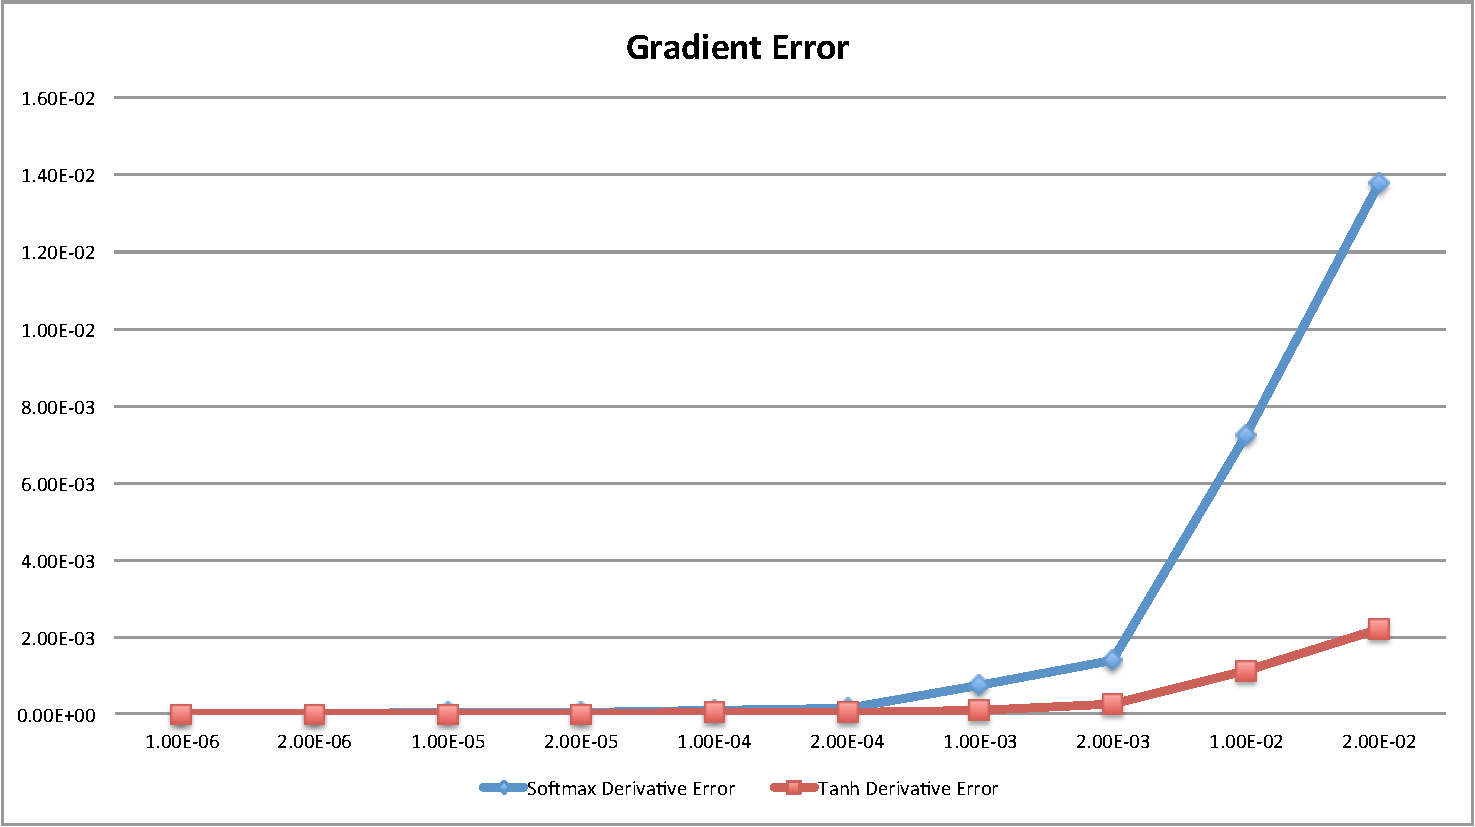
\includegraphics[width=1.\textwidth]{gradError.pdf}
\caption{Absolute difference between the numerical gradient and derivatives we derived in this paper.}
\label{figGradCheck}
\end{figure}

\subsection{Convergence of Model Training}


\subsection{Recongition Performance on Test Set}
To further test the 

\section{Discussion}



\begin{thebibliography}{9}
\bibitem{fastlda}
Porteous, Ian, et al. "Fast collapsed gibbs sampling for latent dirichlet allocation." Proceedings of the 14th ACM SIGKDD international conference on Knowledge discovery and data mining. ACM, 2008.


\bibitem{harmonic}
Newton, Michael A., and Adrian E. Raftery. "Approximate Bayesian inference with the weighted likelihood bootstrap." Journal of the Royal Statistical Society. Series B (Methodological) (1994): 3-48.
APA	

\bibitem{wallach}
Wallach, Hanna M., et al. "Evaluation methods for topic models." Proceedings of the 26th Annual International Conference on Machine Learning. ACM, 2009.

\bibitem{pang2002}
Pang, Bo, Lillian Lee, and Shivakumar Vaithyanathan. "Thumbs up?: sentiment classification using machine learning techniques." In Proceedings of the ACL-02 conference on Empirical methods in natural language processing-Volume 10, pp. 79-86. Association for Computational Linguistics, 2002.

\bibitem{pang2005}
Pang and L. Lee. 2005. Seeing stars: Exploiting class relationships for sentiment categorization with respect to rating scales. In ACL, pages 115�124.

\end{thebibliography}




\end{document}
